%! TeX program = lualatex

\documentclass[11pt]{extarticle}

% Set 1-inch margins
\usepackage[margin=1in]{geometry}

% Set Times New Roman for text and Cambria Math for math fonts
\usepackage{fontspec}
\setmainfont{Times New Roman}

% Use Symbol font for non-alphabetic characters
\usepackage{textcomp}

% Set line spacing to single (no less than single-spacing)
\usepackage{setspace}
\setstretch{1.0}

% Package for handling citations
\usepackage[backend=biber,style=numeric,sorting=none]{biblatex}
\addbibresource{references.bib}

% For inserting images and subcaptions
\usepackage{graphicx,subcaption} 
\usepackage{wrapfig}
\usepackage{svg}

% Begin document
\begin{document}

\textbf{Graduate Research Plan Statement}

\textbf{Introduction and Background:} Category theory is slowly beginning to permeate various ``applied'' disciplines by providing a unique framing of knowledge discovery processes to provide insight into how these processes can be composed together to yield novel knowledge generation. % TEJA: Ask if this topical sentence is stronger now
Central to this ``quiet revolution'' is the idea of compositionality: the characteristic that ``describes and quantifies how complex things can be assembled out of simple parts'' [1] which is a concept ubiquitous across mathematics but is seen acutely in the fundamentals of category theory.
Simply put, category theory studies the ``relationships that exist between things'' which gives one a vantage point to think not on the minutiae of a particular problem but more broadly about how things in a problem space may ``fit together'' (i.e. ``be composed'').
Category theory is primed to take advantage of ideas common across domains such as ``knowledge discovery'', the process of scrutinizing available data to generate novel insight about a particular field or topic. % TEJA: Does this seem natural?

\begin{wrapfigure}{r}{0.3\textwidth}
\centering
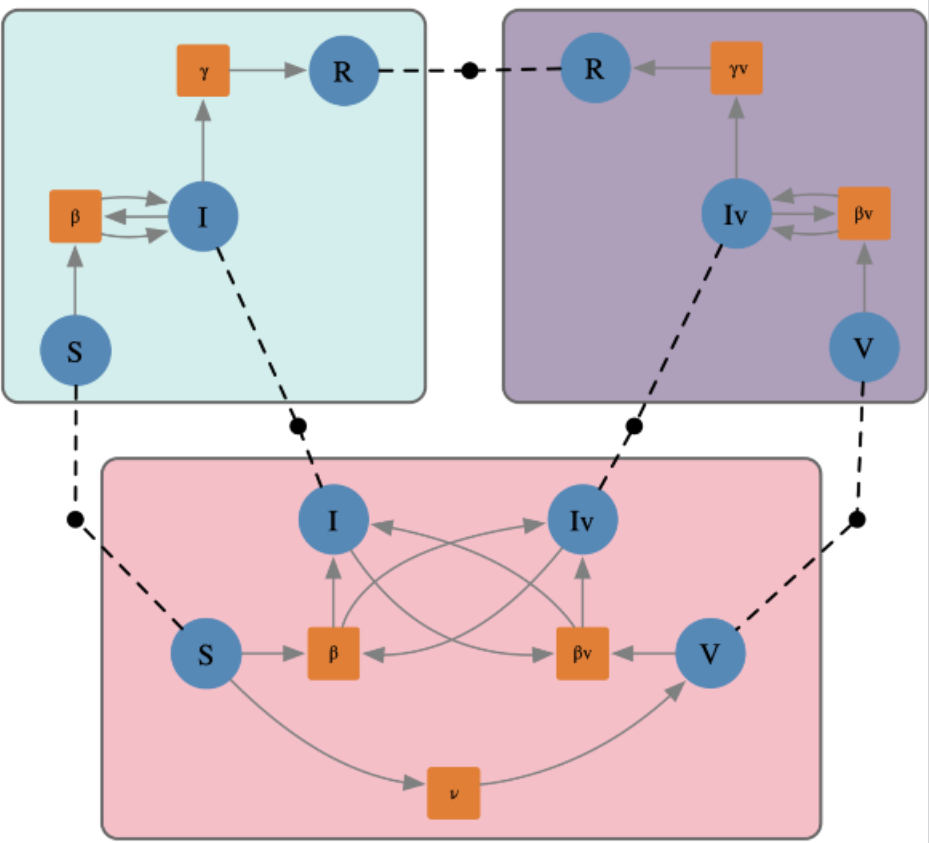
\includegraphics[width=0.3\textwidth]{sub_models}
\vspace{-15pt}
\caption{
  3 discovery processes (the three different petri nets in boxes) with relationships defined by arrows and lines inside of and between processes. % TEJA: How does caption read?
}
\vspace{10pt}
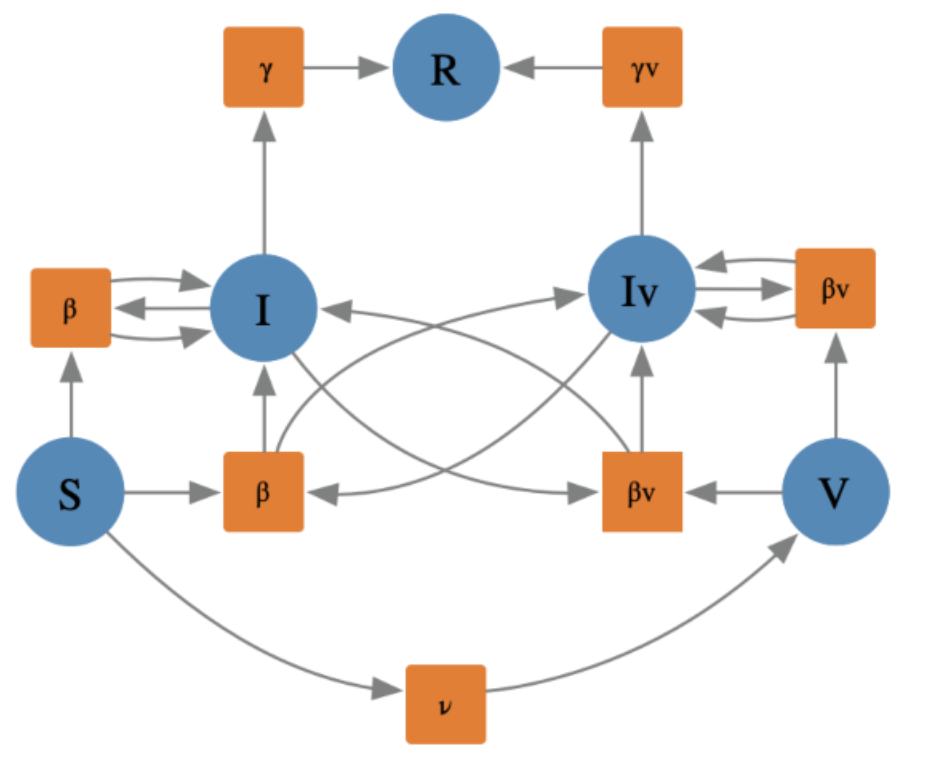
\includegraphics[width=0.25\textwidth]{composed_model}
\vspace{-10pt}
\caption{
  Composition of the 3 discovery processes into one novel discovery process. % TEJA: How does caption read?
}
\end{wrapfigure}

Motivating the objectives of this proposal is my experience within Georgia Tech Research Institute and the US Centers for Disease Control where I noticed that such processes can appear similar across disciplines but due to domain specifics, adapting old proccesses to novel needs can be a laborious and time consuming process. 
To give an example, consider figure 1 which depicts 3 different dynamical systems (denoted by the different figures within each colored box) diagrammed using petri nets, a diagrammatic language well-understood in the terms of category theory. [2]
Within each box, the petri nets are modeling variations of a compartmental model to drive discovery in the context of epidemiology (compartmental models are widespread across epidemiology but have application in economics, ecology, and beyond). 
Here, circles represent populations, squares represent variables that attenuate the strength of the relationships given by arrows between populations, and dotted lines relate populations across the three processes.
Figure 2 then shows the result of how composing these models across dotted lines can reuse separate knowledge discovery processes while also simplifying them into one novel process subsuming former procceses.
\textbf{The goal of this proposal is to demonstrate how category theoretic treatments of knowledge discovery can improve the fundamental understanding of relationships between processes, reduce time needed to find relationships, and how processes can be resused for novel applications.}

\textbf{Research Plan:} At Harvard University, I will pursue a PhD to investigate the category theoretic understanding of knowledge discovery under Professor Nathaniel Osgood.
Additionally, I continue my collaboration relationships with the Topos Institute and the University of Florida GATAS Lab who are pioneering applied category theory approaches and technologies.

\textbf{Objective 1: Map the Knowledge Discovery Process To Category Theoretic Language.} To drive exploration of the general knowledge discovery process, I will pick three heterogeneous data sets that vary by how they are sampled over time and by what kind of data they contain. 
Then, I will construct general knowledge discovery proccesses to scrutinize these data sets through various data science techniques (such as clustering or prediction methods) to simulate deriving novel insights data in general.
After creating these proccesses, I will then explore manually how these data sets could be related to one another.

Once several relationships that could exist within and between data sets have been enumerated, I will then proceed to map these knowledge discovery processes on to various categorical structures.
First, I will use $\mathscr{C}$-sets, which describes a functor mapping a schema category $\mathscr{C}$ into the category $\mathbb{Set}$ (as objects) and functions between them (as morphisms) [3]
Then, to assess how reasonable the identified relationships are, I will use a decorated copresheaf structure (known as "acsets") to compute a presentation of the schema represented by the acset. [4]
This objective will be completed when I have created an adequate $C$-set presentation that describes the relationships present within and between these datasets.

\textbf{Objective 2: Prototype Knowledge Discovery for a Specific Topic Using Category Theoretic Framing.} As the data sets are now framed in category theoretic terms, I will develop a knowledge discovery process for a particular topic beyond what is generally explored with traditional data science approaches using tools from the AlgebraicJulia ecosystem, an open source research software stack based on category theoretic structures. [5]
Using AlgebraicJulia tools, I will determine what metrics and statistics are possible to compute on top of this framing of a knowledge discovery process by taking inspiration from previous work done by Drs. Libkind [2] and Osgood. [6]
Objective 2 will be completed once I have determined what methods are most applicable to this framing and have attempted to formulate questions unique to this categorical framing.

\textbf{Objective 3: Optimizing the Composition of Knowledge Discovery Processes.} At this stage, I will perform objectives 1 and 2 again but to construct a different $C$-set presentation for another knowledge discovery process on top of the same datasets currently being used for investigation.
Once this other knowledge discovery process has been completed, I am now at the arguably most exciting parts of this work: determining how to optimally compose knowledge discovery processes together.
I will define the relationships that can exist throughout these processes (as in figure 1) and then determine how to compose and simplify these processes into a novel discovery process (as in figure 2).
Objective 3 will be completed when I have, in a similar manner to objective 2, determined what metrics I can compute upon this composed structure and determine what novel insight this new process can uncover within the topic of investigation.

\textbf{Intellectual Merit:} By using category theory to frame knowledge discovery involving heterogeneous datasets, data harmonization could become a simpler process versus any manual investigation of data sets via traditional data science practices.
As mentioned in Figures 1 and 2, relationships could be seen much more clearly across discovery processes and one can have an easier way of tracking the complexities of large processes or the compositions thereof with this framing.
In this way, the time cost of understanding and repurposing old processes could be greatly reduced and could lead to quicker insights into new problems rather than in an ad hoc manner of testing various data science methods against a data set or collection of data sets.

\textbf{Broader Impacts:} Category theory has a long history of application with database architecture [7] but is also finding applications within engineering system design [8] and machine learning. [9]
By pursuing this work, I will be at the forefront of these emerging applications and can expand how complex knowledge discovery systems can be understood and analyzed across various disciplines.
Furthermore, this work could improve the construction of discovery processes from inception by allowing one to easily reason through how developing processes could be composed in the future or with other processes while in development leading to these knowledge discovery processes potentially being reduced from weeks to a matter of days. [10]
Finally, as I will be exploring the limits of the available category theoretic machinery through this work, I will be poised to investigate new frontiers in applying category theory whether through informing the foundational mathematics of category theory or in the development of new open source research software that can be reused and developed further within the category theory community.

\textbf{References:} [1] \textit{Compositionality}, 2024. [2] \textit{An Algebraic Framework for Structured Epidemic Modelling.}, Libkind, et. al., 2022. [3] \textit{Categorical Software Engineering for Dynamic Simulation Modeling in Systems Science}, 2024. [4] \textit{Categorical Data Structures for Technical Computing}, Lynch, et. al., 2021. [5] \textit{AlgebraicJulia: a compositional approach to technical computing}, Patterson, 2022. [6] \textit{ModelCollab}, Baez, et. al., 2024. [7] \textit{Algebraic Databases}, Shultz, et. al., 2016. [8] \textit{ACT4ED}, MIT 1.S980, 2024. [9] \textit{Category theory in machine learning}, Gavranović, 2021. [10] \textit{Measuring the impact of knowledge loss: a longitudinal study}, Massingham

\end{document}
